\section{SceneGraph Class Reference}
\label{classSceneGraph}\index{SceneGraph@{SceneGraph}}
{\tt \#include $<$SceneGraph.h$>$}



\subsection{Detailed Description}
This class is the scene graph. 

Definition at line 24 of file SceneGraph.h.\subsection*{Public Member Functions}
\begin{CompactItemize}
\item 
{\bf SceneGraph} (void)
\begin{CompactList}\small\item\em Default constructor. \item\end{CompactList}\item 
{\bf $\sim$SceneGraph} (void)
\begin{CompactList}\small\item\em Default destructor. \item\end{CompactList}\item 
void {\bf addRootNode} (boost::shared\_\-ptr$<$ {\bf SceneGraphNode} $>$ rootNode)
\begin{CompactList}\small\item\em \begin{Desc}
\item[Parameters:]
\begin{description}
\item[{\em rootNode}]The node that will become the node of the scene graph \end{description}
\end{Desc}
\item\end{CompactList}\item 
void {\bf addNode} (boost::shared\_\-ptr$<$ {\bf SceneGraphNode} $>$ parentNode, boost::shared\_\-ptr$<$ {\bf SceneGraphNode} $>$ childNode)
\begin{CompactList}\small\item\em \begin{Desc}
\item[Parameters:]
\begin{description}
\item[{\em parentNode}]The parent node already in the scene graph \end{description}
\end{Desc}
\item\end{CompactList}\item 
boost::shared\_\-ptr$<$ {\bf SceneGraphNode} $>$ {\bf getNode} (vertex\_\-descriptor id)
\begin{CompactList}\small\item\em \begin{Desc}
\item[Parameters:]
\begin{description}
\item[{\em id}]an index of which node to return \end{description}
\end{Desc}
\item\end{CompactList}\item 
std::string {\bf listNodes} (void)
\begin{CompactList}\small\item\em \begin{Desc}
\item[Parameters:]
\begin{description}
\item[{\em outputStream}]an output stream to write a list of nodes in the graphs to \end{description}
\end{Desc}
\item\end{CompactList}\item 
const {\bf graph\_\-type} {\bf getGraph} (void)
\begin{CompactList}\small\item\em \begin{Desc}
\item[Returns:]a graph instance to be traversed by an algorithm \end{Desc}
\item\end{CompactList}\item 
std::string {\bf getDotGraph} (void)
\begin{CompactList}\small\item\em \begin{Desc}
\item[Returns:]a string containing the graph in graphviz dot format \end{Desc}
\item\end{CompactList}\end{CompactItemize}


\subsection{Constructor \& Destructor Documentation}
\index{SceneGraph@{SceneGraph}!SceneGraph@{SceneGraph}}
\index{SceneGraph@{SceneGraph}!SceneGraph@{SceneGraph}}
\subsubsection{\setlength{\rightskip}{0pt plus 5cm}SceneGraph::SceneGraph (void)}\label{classSceneGraph_cd0ba5e308f0d5b54d95522318274579}


Default constructor. 



Definition at line 7 of file SceneGraph.cpp.\index{SceneGraph@{SceneGraph}!$\sim$SceneGraph@{$\sim$SceneGraph}}
\index{$\sim$SceneGraph@{$\sim$SceneGraph}!SceneGraph@{SceneGraph}}
\subsubsection{\setlength{\rightskip}{0pt plus 5cm}SceneGraph::$\sim$SceneGraph (void)}\label{classSceneGraph_9de03f60b86e0ab36a52e9393c8bec01}


Default destructor. 



Definition at line 12 of file SceneGraph.cpp.

\subsection{Member Function Documentation}
\index{SceneGraph@{SceneGraph}!addRootNode@{addRootNode}}
\index{addRootNode@{addRootNode}!SceneGraph@{SceneGraph}}
\subsubsection{\setlength{\rightskip}{0pt plus 5cm}void SceneGraph::addRootNode (boost::shared\_\-ptr$<$ {\bf SceneGraphNode} $>$ {\em rootNode})}\label{classSceneGraph_e6eeea8a739aedc54d8afc8b422766e9}


\begin{Desc}
\item[Parameters:]
\begin{description}
\item[{\em rootNode}]The node that will become the node of the scene graph \end{description}
\end{Desc}


\begin{Desc}
\item[Warning:]there can only be one root node add a root node \end{Desc}


Definition at line 16 of file SceneGraph.cpp.

Referenced by BOOST\_\-AUTO\_\-TEST\_\-CASE().

Here is the caller graph for this function:\nopagebreak
\begin{figure}[H]
\begin{center}
\leavevmode
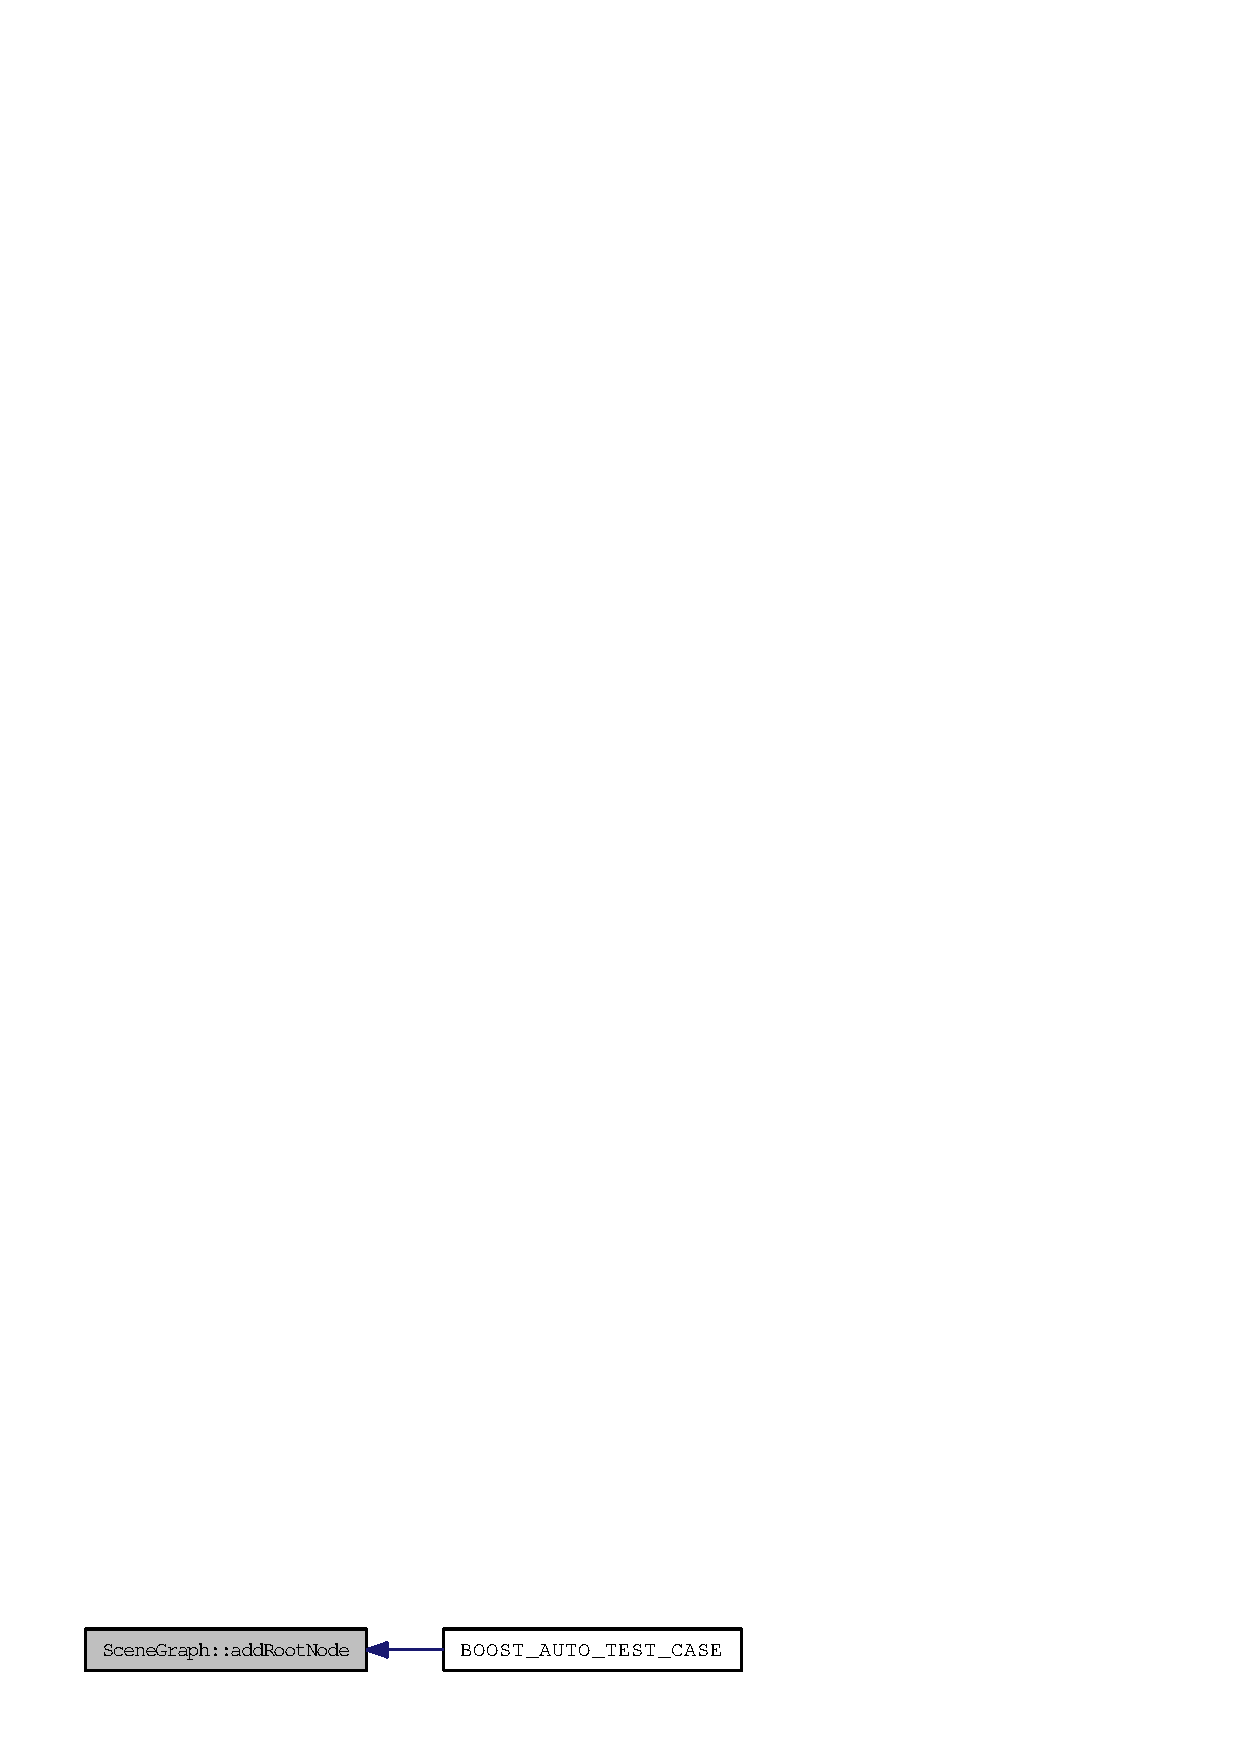
\includegraphics[width=180pt]{classSceneGraph_e6eeea8a739aedc54d8afc8b422766e9_icgraph}
\end{center}
\end{figure}
\index{SceneGraph@{SceneGraph}!addNode@{addNode}}
\index{addNode@{addNode}!SceneGraph@{SceneGraph}}
\subsubsection{\setlength{\rightskip}{0pt plus 5cm}void SceneGraph::addNode (boost::shared\_\-ptr$<$ {\bf SceneGraphNode} $>$ {\em parentNode}, boost::shared\_\-ptr$<$ {\bf SceneGraphNode} $>$ {\em childNode})}\label{classSceneGraph_1c6ad1ade4f196573a0348fdab924bb0}


\begin{Desc}
\item[Parameters:]
\begin{description}
\item[{\em parentNode}]The parent node already in the scene graph \end{description}
\end{Desc}


\begin{Desc}
\item[Parameters:]
\begin{description}
\item[{\em childNode}]The child \end{description}
\end{Desc}
\begin{Desc}
\item[Warning:]the parent node must be in the graph already and the child node can not be add a child node to the graph with a specific parent \end{Desc}


Definition at line 33 of file SceneGraph.cpp.

Referenced by BOOST\_\-AUTO\_\-TEST\_\-CASE().

Here is the caller graph for this function:\nopagebreak
\begin{figure}[H]
\begin{center}
\leavevmode

\includegraphics[width=169pt]{classSceneGraph_1c6ad1ade4f196573a0348fdab924bb0_icgraph}
\end{center}
\end{figure}
\index{SceneGraph@{SceneGraph}!getNode@{getNode}}
\index{getNode@{getNode}!SceneGraph@{SceneGraph}}
\subsubsection{\setlength{\rightskip}{0pt plus 5cm}boost::shared\_\-ptr$<$ {\bf SceneGraphNode} $>$ SceneGraph::getNode (vertex\_\-descriptor {\em id})}\label{classSceneGraph_3d8dfec1bb4e175f87c0d44462140244}


\begin{Desc}
\item[Parameters:]
\begin{description}
\item[{\em id}]an index of which node to return \end{description}
\end{Desc}


\begin{Desc}
\item[Returns:]the node indicated by the index \end{Desc}


Definition at line 54 of file SceneGraph.cpp.

Referenced by BOOST\_\-AUTO\_\-TEST\_\-CASE().

Here is the caller graph for this function:\nopagebreak
\begin{figure}[H]
\begin{center}
\leavevmode

\includegraphics[width=168pt]{classSceneGraph_3d8dfec1bb4e175f87c0d44462140244_icgraph}
\end{center}
\end{figure}
\index{SceneGraph@{SceneGraph}!listNodes@{listNodes}}
\index{listNodes@{listNodes}!SceneGraph@{SceneGraph}}
\subsubsection{\setlength{\rightskip}{0pt plus 5cm}std::string SceneGraph::listNodes (void)}\label{classSceneGraph_86ebfcf900443c1b28f9c2a2c2fc8ea8}


\begin{Desc}
\item[Parameters:]
\begin{description}
\item[{\em outputStream}]an output stream to write a list of nodes in the graphs to \end{description}
\end{Desc}




Definition at line 59 of file SceneGraph.cpp.

Referenced by BOOST\_\-AUTO\_\-TEST\_\-CASE().

Here is the caller graph for this function:\nopagebreak
\begin{figure}[H]
\begin{center}
\leavevmode
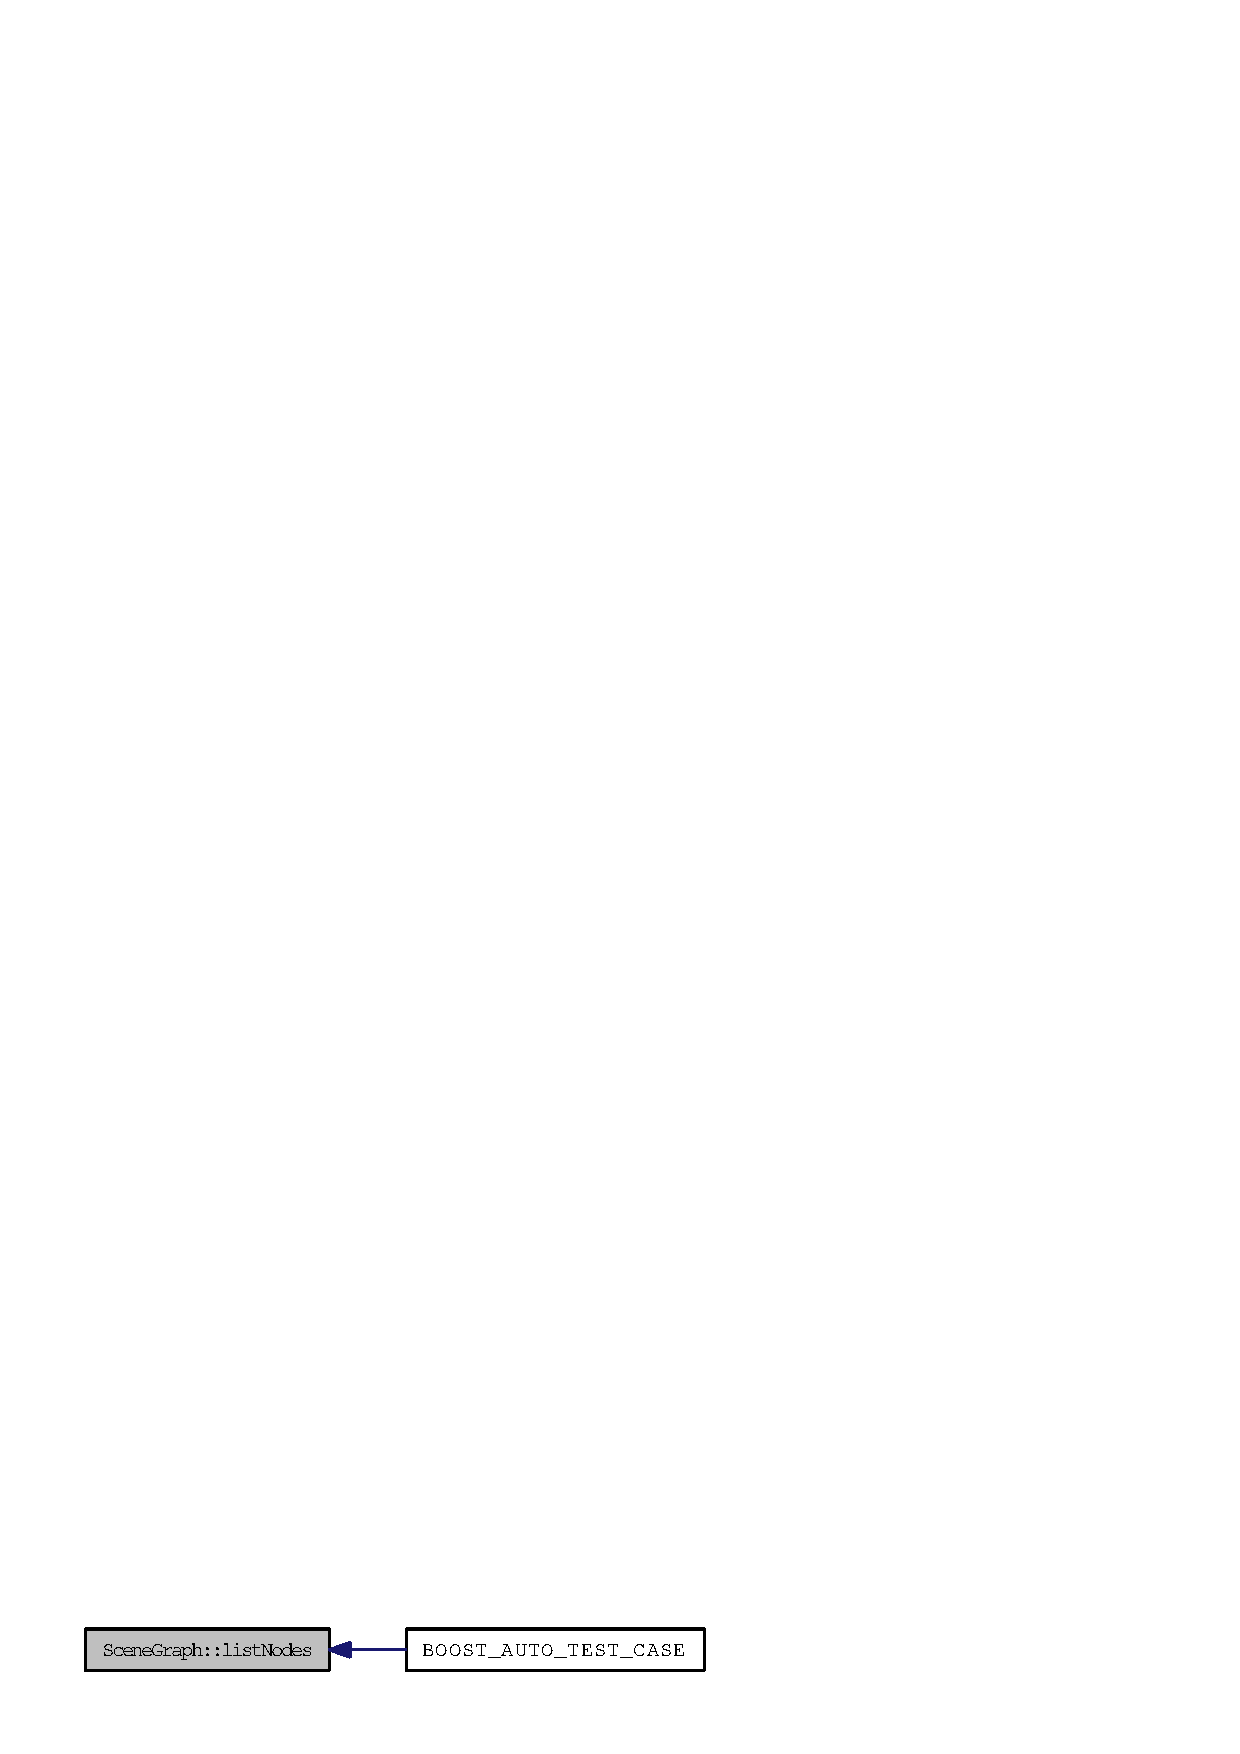
\includegraphics[width=171pt]{classSceneGraph_86ebfcf900443c1b28f9c2a2c2fc8ea8_icgraph}
\end{center}
\end{figure}
\index{SceneGraph@{SceneGraph}!getGraph@{getGraph}}
\index{getGraph@{getGraph}!SceneGraph@{SceneGraph}}
\subsubsection{\setlength{\rightskip}{0pt plus 5cm}const {\bf graph\_\-type} SceneGraph::getGraph (void)}\label{classSceneGraph_0df0b539245afe403114fab4831c045d}


\begin{Desc}
\item[Returns:]a graph instance to be traversed by an algorithm \end{Desc}




Definition at line 72 of file SceneGraph.cpp.\index{SceneGraph@{SceneGraph}!getDotGraph@{getDotGraph}}
\index{getDotGraph@{getDotGraph}!SceneGraph@{SceneGraph}}
\subsubsection{\setlength{\rightskip}{0pt plus 5cm}std::string SceneGraph::getDotGraph (void)}\label{classSceneGraph_5eee36560f2b6c1d7b8717feaf46503b}


\begin{Desc}
\item[Returns:]a string containing the graph in graphviz dot format \end{Desc}




Definition at line 79 of file SceneGraph.cpp.

The documentation for this class was generated from the following files:\begin{CompactItemize}
\item 
{\bf SceneGraph.h}\item 
{\bf SceneGraph.cpp}\end{CompactItemize}
